\chapter{Existing solutions}
\todo[inline]{write that there are figures - screenshots in each app}
In this chapter we will discuss currently available solutions in our problem domain.
First, each application is briefly introduced.
Second, we state use cases by which we later compare the applications.
Last, we describe how each application fulfills these use cases.

\section{Overview of existing similar applications}
Now we will briefly introduce currently available applications.

% osnova popisovania aplikacie:
% uvodne predstavenie, ako sa s nou pracuje, vyhody (co aplikacia nesplna popisat v comparison of apps), dalsie zaujimavosti
\todo[inline]{add link in footnote}
\subsection*{Allergy Menu}
  Allergy menu allows a restaurant employee to maintain a mobile accessible and up-to-date menu that customers can tailor to their food preferences.
  
  A restaurant employee first creates a new menu and adds categories to it, e.g. "Starters" or "Desserts".
  Dishes are then added to each category of the menu.
  A dish contains allergen information as well as flags whether it is suitable for vegans and vegetarians.
  The restaurant employee can also add calories to the dish.

  When a restaurant employee wants to change something in a dish, they can create a copy of the dish which is hidden on the published menu.
  After they finish changes, the dish can be marked as "live", making it appear on the menu with updated content. 

  A dish can optionally contain internal notes, with the ability to upload photographs of products used within the dish.
  The application sends and e-mail regularly to review a menu with all the allergy information.
  An existing menu can be imported to the application in the CSV format.
  Allergy Menu provides an API for food suppliers, allowing them to sync menu information directly into the application without manual intervention.
  
  A guest can interact with a published menu by choosing what allergens they want to avoid.
  The application then filters out items of the menu to meet the guest's preferences.
  A guest can also select an option that they are either a vegan or vegetarian.
  
  A unique restaurant code is used to identify restaurants. 
  This is what guests enter into the application when they want to browse a menu.
  A guest can also find a restaurant which uses Allergy Menu on a map.
  \todo[inline]{a restaurant can only have one menu published - mention in comparison}

  \newpage

  \begin{figure}[h]
    \centering
    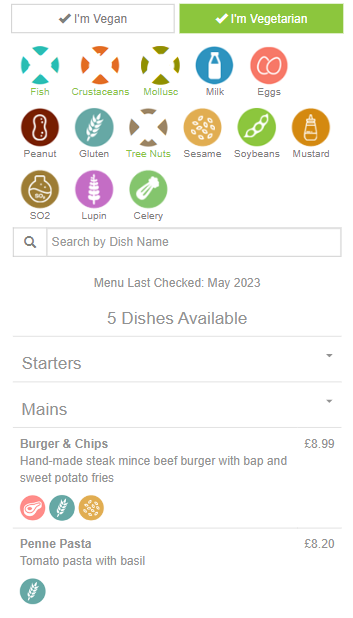
\includegraphics[height=12cm]{master-thesis/img/existing-applications-screenshots/allergy_menu_screenshot}
    \caption{The Allergy Menu application}
  \end{figure}
% end of \subsection

\todo[inline]{add link in footnote}
\subsection*{Allergen Checker}
  Allergen Checker is an allergen management software which enables a restaurant employee to add allergen information to a menu.
  
  A menu is created in three steps.
  In the first step, the restaurant employee creates ingredients which are then stored in a database called the restaurant's "virtual food cupboard".
  During the second step, the restaurant employee creates dishes by specifying their ingredients.
  In the third step, the restaurant employee creates a menu by specifying its dishes.
  
  The application provides a pre-defined list of basic ingredients in its database.
  An ingredient has information about what allergen it contains and also what allergens it may contain. 
  The restaurant employee can also copy information from the ingredient's packaging which will be then displayed in a dish's description in the menu.
  
  Allergen Checker allows for categorizing of dishes and menus. 
  Categories are thought of as a file system for dishes and menus.
  This is convenient when the restaurant employee needs to search for a specific menu or dish.

  \begin{figure}[h]
    \centering
    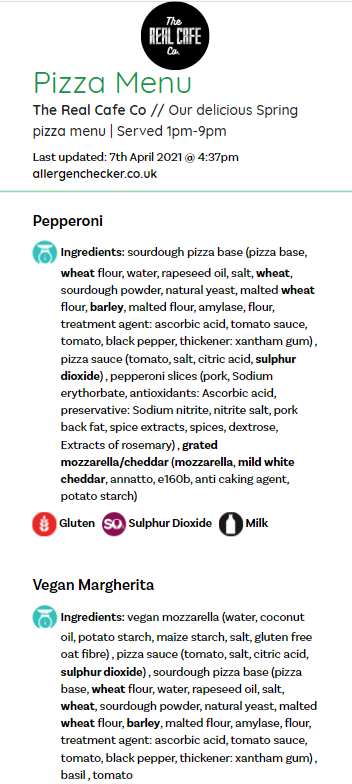
\includegraphics[height=12cm]{master-thesis/img/existing-applications-screenshots/allergen_checker_menu_screenshot}
    \caption{The Allergen Checker application}
  \end{figure}
% end of \subsection

\todo[inline]{add link in footnote}
\subsection*{BigZpoon Eagle}
  BigZpoon Eagle provides preference-based allergen and nutrition menus for \linebreak restaurants.
  It is a cloud-based SaaS solution which and two parts.

  One part is the consumer-facing website.
  It allows a restaurant's guest to set their dietary restrictions and nutritional goals.
  After this is done, a personalized menu is presented to the guest.
  Items of a menu are shown in three groups.
  There are items which are "Okay to eat", items which are "Okay to eat with modifications" and items which are "Not okay to eat".
  Items and ingredients which are not okay to eat are clearly marked in the item's detail.
  
  The application also supports online ordering of meals.
  The guest can select what they want to eat and choose different ingredients.
  The Eagle platform tries to recommend to the guest what they might want to order using a sort of artificial intelligence algorithm.
  The application also displays detailed nutritional information for the current state of the order and shows whether the guest's nutritional goals are met.

  The consumer-facing website sends analytical data to the backend portal application, which is the other part of the Eagle platform.
  It serves for restaurants to manage their online menus and see insights on how their customers are using the guest application.
  The portal allows creating multi-location menus to show a different menu based on the restaurant's location.
  The restaurant employee can set up menu groups, categories and individual food items.
  A menu item can be disabled for a certain category, group or restaurant location.
  Creating a menu item involves adding all choices and their variations.
  A restaurant employee can manually create restaurant ingredients or choose from a pre-defined list of ingredients.

  \begin{figure}[h]
    \centering
    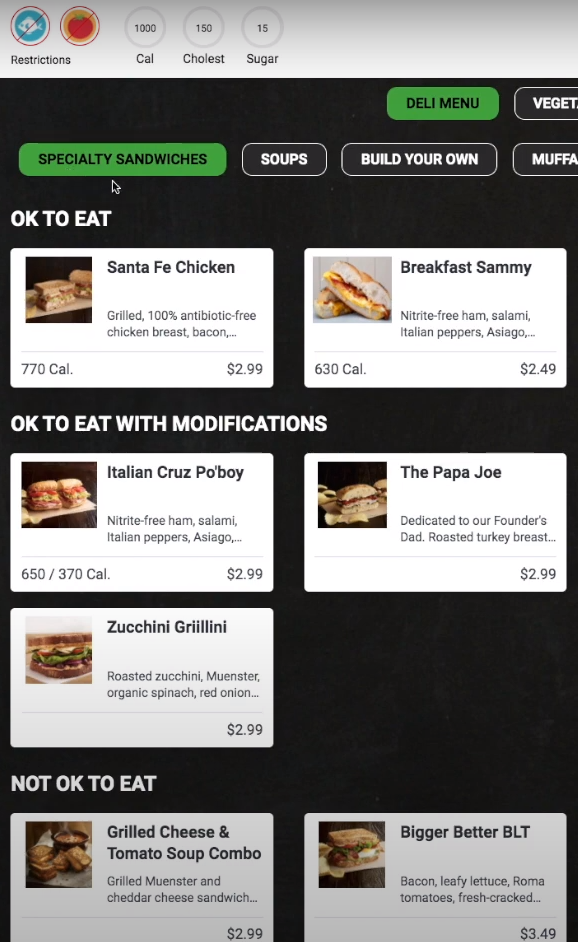
\includegraphics[height=12cm]{master-thesis/img/existing-applications-screenshots/bigzpoon_screenshot}
    \caption{The BigZpoon application}
  \end{figure}
% end of \subsection

\newpage

\subsection*{Tenkites}
  can link to existing EAS and POS system
  information to tenkites and out to every point of sale
  can be connected to social media
  optimized for search engines
  dashboard insights

  \begin{figure}[h]
    \centering
    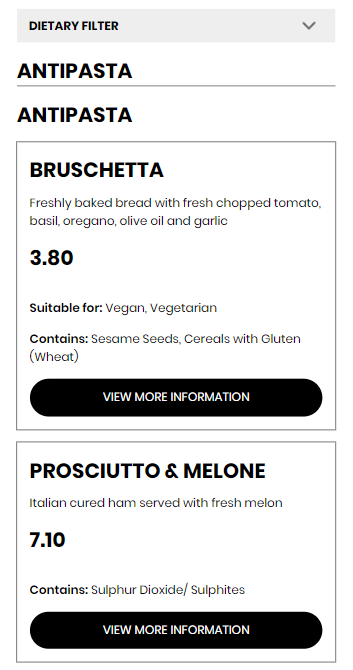
\includegraphics[height=12cm]{master-thesis/img/existing-applications-screenshots/tenkites_menu_screenshot}
    \caption{The Tenkites application}
  \end{figure}
% end of \subsection

\subsection*{Menu Guide}
% Intro
  Menu Guide is a tool used to maintain accurate, recorded allergen and dietary information, and to share those with staff and customers through customized, interactive pages.
% Menu creation
% Item creation
  When creating a new menu, a restaurant employee adds items to it. 
  An item can be a food item or for example a heading for a category name.
  A food item has information like name, price, calories and a list of ingredients as plain text.
  The restaurant employee can specify the item's allergens.
  An item can be set to contain, may contain or trace an allergen.
  When ingredients are inserted, the application automatically highlights ingredients which contain allergens.
  Some allergens like nuts contain sub-allergens to choose from, for example almond or cashew.
  A food item can be marked as vegan or vegetarian.
  If the restaurant employee selects the vegan option and the item already contains milk as its allergen, the app will warn the restaurant employee that they made a mistake.
  
  % other menu stuff

  Restaurant employee can set a customer message which is displayed upon loading a menu.
  There is a standard message and optionally restaurant employee can add additinal information to this message.

  restaurant employee can choose from several design templates when creating a menu or apply your own custom styling using CSS

  restaurant employee can schedule when a menu will be active and when it will be deactivated

  restauran employee can select that a menu will be active repeatedly for specific days

  restaurant employee can select whether a menu is published

  autosave when creating a menu

  restaurant employee can view and restore previous versions of a menu 

  preview of menu - how it will look when published
  click to open a new window (desktop or tablet only) showing how your menu will look once approved and published online

  restaurant employee can select for which business a menu will be created for

  A menu can be uploaded directly from a website, menu pdf, the restaurant's own allergen sheet, or from a built-in allergen menu spreadsheet. 

  Restaurant employee can choose to upload a menu using a pre-defined CSV spreadsheet template.
  Menu Guide accepts Microsoft Word, Excel, CSV and Powerpoint, Adobe PDF and Apache
  OpenOffice document formats. Click on the ‘Upload my menu’ button to open a new
  window, select your menu and click ‘open’
  CSV template users can map their template fields to Menu Guide fields
  Let Menu Guide fetch your menu from your website: enter the URL (website address) of your menu and click on the ‘Get menu’ button.
% Linked menus
  restaurant employee has options to create linked menus - they can have the same menus with different QR code in multiople areas - a master menu - rtestaurant employee only edits the master menu and other menus are also updated automatically

  employee can publish new menu to an existing short link or create a new short link 

  Shortlink (mnu.mx/xxxx) – this converts the URL (website address) of your Menu Guide
  page into a shorter, user-friendly format. Click on the shortlink to see your menu navigation page open in a new window, with the menu that you have just created.

  deletion of a parent menu will delete also the linked menus

  a short link points to a menu list of a restaurant and the apllication is able to generate a QR code for the short link - random numbers or unique string
% Menu active period
  menu expires in a month for safety reasons

  To help keep your content up to date, Menu Guide will send you an email every two months asking you
  to check and confirm that your menus are correct. If you do not act on this request, your menus will
  automatically expire.
% Other
  Save commonly used menu items into a library for re-use in future. 

  restaurant employee can download a menu in csv format 

  see an overview of diner
  activity (total page views and average view duration), a daily breakdown of page views and the allergens and dietary preferences selected by diners.

  No internet of WiFi in your venue? No problem, simply download our offline menus app to a shared tablet (available for Android devices on Google Play) and your customers can browse your allergen menus no matter where they are!

  restaurant employee can print a menu








  restaurant guest can select to remember their dietary preferences

  guest can display menu in a grid

  when a guest opens the app, they see a list of the restaurant's menus and the restaurant message

  no download of app needed

  you may choose to highlight food items that are dairy-free, vegetarian and vegan

  select allergens and the app highlights affected dishes

  \begin{figure}[h]
    \centering
    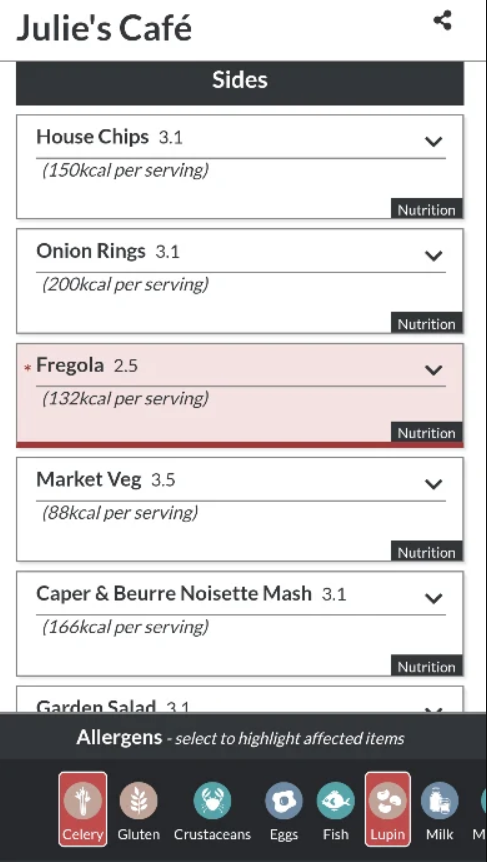
\includegraphics[height=12cm]{master-thesis/img/existing-applications-screenshots/menu_guide_screenshot}
    \caption{The Menu Guide application}
  \end{figure}
% end of \subsection

\todo[inline]{add Hubl app and restaurantallergens.com}
% \subsection*{Hubl}  

  % \begin{figure}[h]
  %   \centering
  %   \includegraphics[width=0.62\linewidth]{master-thesis/img/existing-applications-screenshots/.png}
  %   \caption{The  application}
  % \end{figure}
% end of \subsection